\section{Introduction}
Feed-forward multi-view reconstruction models \citep{wang2025vggt, wang2025pi, depthanything3, wang2026vggtomega, dust3r_cvpr24} regress camera poses and dense geometry directly, without the iterative correspondence-based estimation used by classical structure-from-motion (SfM) \citep{structurefrommotion1, structurefrommotion2, structurefrommotion3}. Their strong performance on standard multi-view benchmarks, however, does not necessarily translate to robustness under the diverse conditions encountered in real-world image capture \citep{liu2026realx3d}. One such source of variability is camera orientation, which can vary substantially across handheld photography, egocentric video capture, and other settings with unconstrained camera motion \citep{xian2019uprightnet}. Classical SfM pipelines are inherently robust to such changes because their geometric estimation relies on rotation invariant image features \citep{SIFTpaper}. For feed-forward reconstruction models, however, robustness to camera orientation is generally assumed as an inherent property of the reconstruction task.

We put this assumption to the test by asking a simple question: \emph{How robust are modern feed-forward reconstruction models to changes in image orientation?} 
A well-behaved reconstruction model should produce point clouds invariant to such changes, while camera poses should transform equivariantly.
Surprisingly, we find that applying random planar rotations on subset of input images leads to degradation in camera pose estimation and dense reconstruction across state-of-the-art (SOTA) feed-forward models. 
We observe this degradation across VGGT \citep{wang2025vggt}, VGGT-$\Omega$ \citep{wang2026vggtomega}, $\pi^3$ \citep{wang2025pi}, MapAnything (MapA.) \citep{keetha2026mapanything} and Depth Anything 3 (DA3) \citep{depthanything3}, while classical SfM with COLMAP \citep{colmap} remains robust to the same perturbations.
Quantitatively, \Cref{fig:baseline_performance}(a) shows that both Absolute Trajectory Error (ATE) and Relative Pose Error (RPE) increase with the number of rotated input images across the feed-forward models. The corresponding qualitative degradation in reconstructed geometry is shown in \Cref{fig:baseline_performance}(b)
We further investigate the extent of this orientation sensitivity across rotations about all three axes (roll, pitch, and yaw) in \cref{sec:how_severe_is_upright_bias}.

We refer to this sensitivity to camera orientation as \emph{UprightBias}: the tendency of feed-forward reconstruction models to perform substantially better on images presented in a canonical upright orientation. The effect is particularly striking because it persists across architecturally diverse models, including reference-view attention networks (VGGT, VGGT-$\Omega$), reference-free permutation-equivariant approaches ($\boldsymbol{\pi^3}$), generalized multi-view matchers such as MapA. and DA3.
% This behavior is particularly striking because it persists across substantially different architectural designs, including reference-view attention models (VGGT, VGGT-$\Omega$), reference-free permutation-equivariant networks ($\boldsymbol{\pi^3}$), and generalized multi-view matchers such as MapAnything (MapA.) \citep{keetha2026mapanything} and DA3. 
% Given how different these designs are from one another, the shared sensitivity is unlikely to stem from any common architectural inductive bias; however,
% Despite the differences, these models exhibit similar sensitivity to image orientation, suggesting that it is unlikely to arise from architectural inductive bias.
Notably, however, each of these models relies on large-scale 3D reconstruction datasets which predominantly consists of canonically-upright images, and models trained on such image sets may potentially learn orientation-specific regularities instead of generalizing across arbitrary rotations.
% -orientation which raises the possibility that the training-data distribution contributes to this behavior. In particular, models may learn orientation-specific regularities prevalent in predominantly canonical training images, rather than developing robustness to arbitrary image rotations.
We investigate this hypothesis through an audit of the training data used by these models in ~\cref{ssec:data_audit}, which shows that an overwhelming majority of these datasets consist of images that are upright by construction, spanning indoor RGB-D benchmarks, outdoor photo collections, and a range of other sources. 

One natural remedy to fix the Upright Bias would be to rebalance the training data with rotated multi-view images and corresponding geometric annotations \citep{redistributingtrainingdata1, tang2022invarianttrainingdata2, kang2019decouplingtrainingdata3}; however, these feed-forward models are built on pretrained visual backbones like DINO-v2/v3 \citep{oquab2023dinov2, simeoni2025dinov3}, and fine-tuning on a rotation-heavy distribution shifts the backbone away from its pretraining regime, which is known to distort learned representations, even when the fine-tuning objective is otherwise met \citep{kumar2022finetuningchallenges, tang2020longchallenges, kang2019decouplingtrainingdata3, horizontalprior}. Further, despite both DA3 and VGGT-$\Omega$ employing $90^\circ$ rotation augmentation in their training pipeline, yet, as shown in \Cref{fig:baseline_performance}(a), they \textit{still exhibit} substantial degradation under arbitrarily-rotated inputs. For instance, we observe that a simple fine-tuning of $\pi^3$ on arbitrarily-rotated training images yields not just inconsistent but often degraded performance (see \cref{sec:training_data_rebalancing} of the supplementary), further suggesting that rebalancing the training distribution \textit{alone} is insufficient to eliminate the upright bias. 
% To probe this further, we fine-tune \textbf{$\pi^3$} on arbitrarily-rotated input images, with results reported in the supplementary \cref{sec:training_data_rebalancing}.
% The resulting model shows inconsistent and often degraded performance under rotated inputs, suggesting that retraining with rotated data alone is insufficient to eliminate this bias.
% Notably, both DA3 and VGGT-$\Omega$ incorporate $90^\circ$ rotation augmentation during training, yet still exhibit substantial degradation under rotated inputs, directly demonstrating that augmentation alone is insufficient to resolve \textcolor{green}{[Abhipsa: is calling it like a proper noun always necessary? :P ]}UprightBias. 
% We empirically validate these limitations further in the supplementary \cref{sec:training_data_rebalancing}, where fine-tuning $\pi^3$ on rotated data confirms inconsistent, often degraded performance rather than resolving UprightBias.
Lastly, we note that retraining large-scale feed-forward models requires \textit{paired} rotated multi-view data with ground-truth geometry, which is currently missing in the existing benchmarks. 

\begin{figure}[t]
    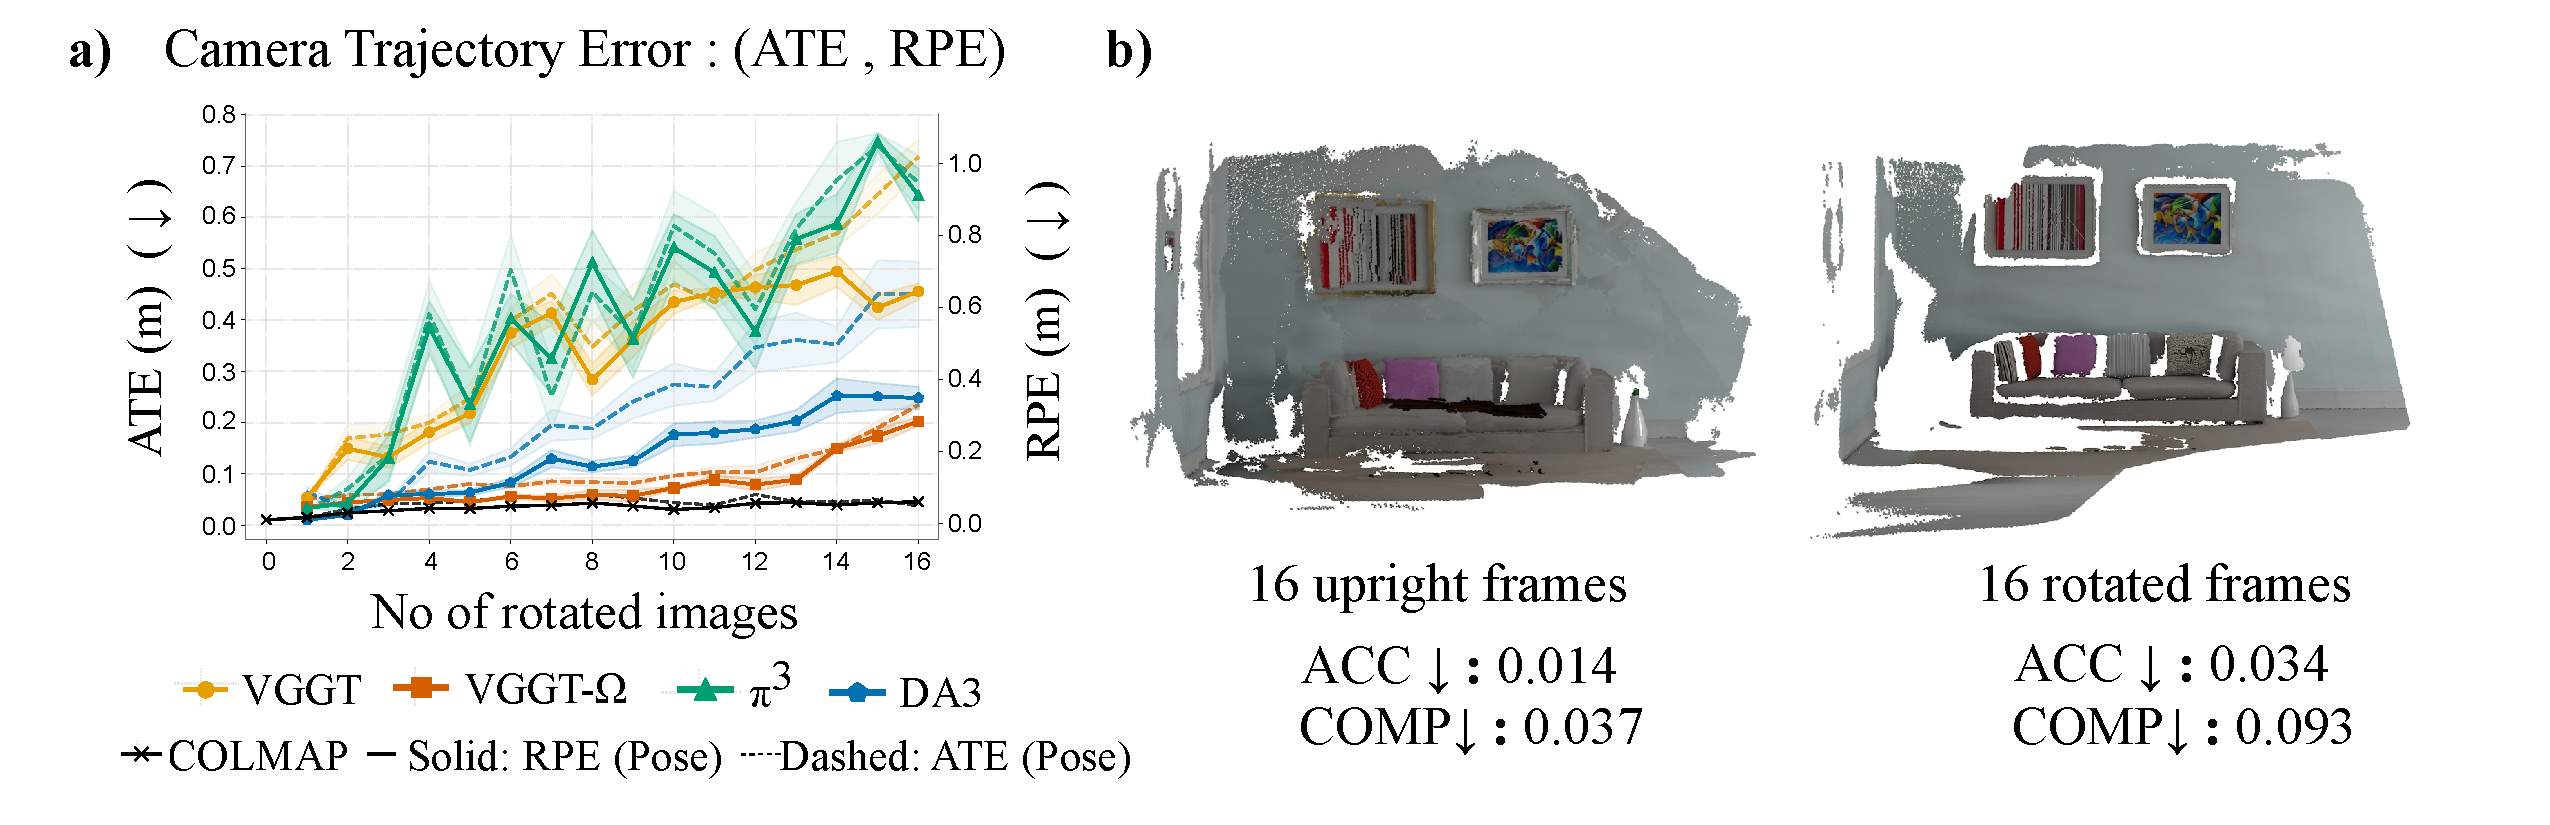
\includegraphics[width=\linewidth]{Figures/fig2/fig2.pdf}
    \caption{\textbf{Robustness against in-plane rotations:}
    (a) Camera poses error increases as number of rotated input images increases ($\theta \sim \mathcal{U}(0^\circ, 360^\circ)$). (b) Qualitative 3D reconstruction degradation on VGGT-$\Omega$ when introducing 16 rotated images sampled from $\theta \sim \mathcal{U}(0^\circ, 360^\circ)$.}
    \label{fig:baseline_performance}
    \vspace{-3mm}
\end{figure}

Rather than adapting a reconstruction model to rotated inputs, we instead ask whether the inputs \textit{themselves} can be rectified to the canonical orientation before reconstruction.
This requires a visual representation that can provide a reliable signal of image orientation without rotation labels or model retraining. To this end, we find that DINOv2 token embeddings exhibit \textit{systematic orientation-dependent variation}, which can be leveraged to enable zero-shot rectification by identifying the orientation that maximizes feature variance. Building on this observation, we propose \textbf{ROVER} (\textbf{RO}tation estimation via \textbf{V}ariance-based \textbf{E}mbedding \textbf{R}ectification), a lightweight \textit{training-free} framework that operates at inference time in a plug-and-play manner with any encoder, as illustrated in ~\cref{fig:teaser}.
% \sout{Along with this, we also introduce \textbf{RotMV} (\textbf{Rot}ational \textbf{M}ulti-\textbf{V}iew), an evaluation benchmark comprising multi-view sequences captured at systematically varied camera orientations to assess rotation-invariance of feed-forward models under real-world scene conditions} \textcolor{red}{[Priyam: any specifics of the benchmark?]}.
Along with this, we introduce \textbf{RotMV} (\textbf{Rot}ational \textbf{M}ulti-\textbf{V}iew), a real-world benchmark comprising of seven multi-view sequences captured across $16$ viewpoints and $12$ in-plane camera orientations spanning $360^\circ$, enabling systematic evaluation of rotation-invariance in feed-forward models.
Extensive Experiments on 7-Scenes, NRGB-D, DTU, ETH3D, Mip-NeRF 360, Tanks \& Temples and RotMV, shows that ROVER recovers reconstruction quality under arbitrary planar rotations while preserving performance on canonical inputs.
% To enable such a training-free approach, we seek a visual representation that provides information about image orientation and can therefore serve as a signal for estimating the canonical orientation of the input.
% We find that DINOv2 token embeddings exhibit a strong orientation signal, with feature variance maximized at the canonical orientation, enabling zero-shot orientation estimation without prior knowledge of the applied rotations or model retraining.
% Leveraging this observation, we propose \textcolor{orange}{[Priyam: I'm not sure if we need to bold ROVER, as well as de-acronymize it here, although it's a choice of writing taste]} \textbf{ROVER} (\textbf{RO}tation estimation via \textbf{V}ariance-based \textbf{E}mbedding \textbf{R}ectification), a lightweight training-free framework that canonicalizes rotated inputs before reconstruction. 
% \textcolor{orange}{[Priyam: This line of RotMV (please give a better name) disconnects with the prev. para about no dataset existing for rotated imgs with geometry info]} \textcolor{green}{[Abhipsa: I feel this line's construction could be improved. Like to the best of our knowledge, we are the first to introduce..., also make it clear that it is an eval dataset]} Since no existing benchmark provides paired upright and rotated multi-view sequences under real-world capture conditions, we introduce \textbf{RotMV}, a curated dataset of real-world multi-view sequences with systematically varied orientations to support controlled evaluation of rotation robustness. Extensive experiments show that ROVER consistently recovers 3D reconstruction quality under arbitrary planar rotations while preserving performance on canonical inputs.
In summary, our main contributions are:

$\bullet$ We identify a previously uncharacterized sensitivity to image orientation in state-of-the-art feed-forward 3D reconstruction models, a phenomenon we term UprightBias, and show that it is systemic across diverse model architectures and families.

$\bullet$ To address it, we propose ROVER -- a lightweight, training-free framework that rectifies input rotations at inference time using orientation-dependent variance in DINOv2 embeddings.

% $\bullet$ \textcolor{orange}{[Priyam: This contribution is currently in a very bad shape (writing-wise). Also check the natural order of the contributions, if they make sense in the current ordering in which they're mentioned]} \Badri{Proper motivation of introducing RotMV is missing, we should use "controlled rotation synthesis" as synthetic and need real data} 
% \textcolor{blue}{We extensively evaluate rotation robustness across six existing datasets through controlled rotation synthesis. Furthermore, we introduce \textbf{RotMV}, a real-world benchmark with paired upright and rotated multi-view sequences, to further validate our findings under real-world camera rotations.}

$\bullet$ Across six existing multi-view datasets, we conduct a systematic assessment of rotation-invariance of various feed-forward models under controlled rotation synthesis, isolating the effect of camera orientation on reconstruction.

$\bullet$ To complement synthetic evaluation with real-world data, we introduce RotMV, a benchmark comprising paired upright and rotated multi-view sequences captured under systematically varied camera orientations.
